\chapter{Marco Lógico del Proyecto}\label{cap:marco-logico}
El marco lógico organiza la relación entre el contexto que motiva el trabajo, el problema que se pretende resolver, las razones que justifican la intervención y los objetivos verificables que orientan cada fase del desarrollo. En este capítulo se presenta primero la contextualización y los antecedentes del proyecto; a continuación, el planteamiento del problema, apoyado en un árbol de problemas; luego, la justificación desde las perspectivas técnica, académica, social y de viabilidad; y, finalmente, el objetivo general y los objetivos específicos que se contrastan en los Capítulos~\ref{cap:implementacion} y~\ref{cap:conclusiones}.

\section{Contextualización y antecedentes}\label{sec:contexto}
La inteligencia artificial (IA) dejó de ser un campo de investigación especializado para convertirse en una tecnología transversal que hoy interviene en el diagnóstico médico, la logística, la agroindustria, la educación y los servicios públicos. Su núcleo técnico más difundido son las redes neuronales artificiales, cuya historia se remonta al modelo lógico de neurona propuesto por \citet{mcculloch1943} y al perceptrón de \citet{rosenblatt1958}. El entusiasmo inicial por estos modelos se frenó cuando \citet{minsky1969} demostraron que un perceptrón de una sola capa no puede representar funciones que no sean linealmente separables, siendo la compuerta XOR el ejemplo más conocido. El campo resurgió con la difusión del algoritmo de retropropagación del error \citep{rumelhart1986} y con los resultados teóricos que establecen que una red con al menos una capa oculta es un aproximador universal de funciones continuas \citep{cybenko1989,hornik1989}. Desde la década de 2010, el aprendizaje profundo ha transformado la visión por computador, el procesamiento del lenguaje natural y numerosos dominios científicos \citep{lecun2015,goodfellow2016,russell2021}.

Este crecimiento ha tenido un efecto ambivalente en la formación de ingenieros. El informe \emph{AI Index} de la Universidad de Stanford documenta el aumento sostenido de la inversión, de las publicaciones y de los modelos de IA a escala mundial, pero también la concentración de su desarrollo en un número reducido de organizaciones con gran capacidad de cómputo \citep{maslej2024}. La UNESCO, por su parte, ha subrayado que las instituciones educativas deben formar personas capaces de comprender críticamente los sistemas de IA y no únicamente de utilizarlos \citep{unesco2022}. Entre ambos diagnósticos aparece una brecha formativa concreta: una gran cantidad de usuarios emplea \emph{frameworks} de alto nivel como cajas negras, mientras que comparativamente pocos desarrolladores dominan el álgebra lineal, el cálculo diferencial y la optimización numérica que explican por qué y cómo aprende una red neuronal \citep{deisenroth2020}. Un estudiante que entrena un modelo con tres líneas de código puede obtener un resultado aceptable, pero difícilmente podrá diagnosticar por qué una red no converge, por qué una tasa de aprendizaje excesiva satura las neuronas o por qué una arquitectura de una sola capa fracasa ante un problema no lineal.

En paralelo, la ingeniería de sistemas ha incorporado nuevos lenguajes que buscan conciliar rendimiento y seguridad. Rust combina la eficiencia de C y C++ con garantías de seguridad de memoria verificadas en tiempo de compilación, sin recurrir a un recolector de basura \citep{matsakis2014,klabnik2023}. La solidez formal de su modelo de propiedad fue demostrada en el proyecto RustBelt \citep{jung2018}, y la encuesta anual de desarrolladores de Stack Overflow lo ha ubicado de forma reiterada como el lenguaje más admirado por quienes lo utilizan \citep{stackoverflow2024}. Estas propiedades lo vuelven atractivo para construir componentes numéricos de alto rendimiento y, al mismo tiempo, para enseñar disciplina de programación: el compilador obliga a declarar explícitamente quién posee cada dato, quién puede modificarlo y cómo se tratan los errores.

Bolivia participa de esta transformación desde un marco normativo que reconoce el acceso a las tecnologías de información y comunicación como un servicio de interés público y promueve el uso de software libre y estándares abiertos en el Estado, según la Ley N.º~164 \citep{bolivia2011}. Ese marco favorece iniciativas académicas que, como la presente, se basan íntegramente en herramientas abiertas y gratuitas. La transformación digital del país requiere profesionales capaces de comprender, adaptar y mantener tecnología, no solo de consumirla; en el campo de la IA, esto significa formar ingenieros que entiendan los fundamentos de los modelos que utilizan y que puedan construir soluciones propias cuando las herramientas importadas no se ajustan a las restricciones locales de conectividad, presupuesto o hardware.

Santa Cruz, como el departamento de mayor dinamismo económico del país, concentra una parte importante de la actividad empresarial y de servicios, y su ecosistema tecnológico incluye empresas de desarrollo de software, emprendimientos digitales y comunidades técnicas que organizan talleres y encuentros de programación. En ese entorno, los productos basados en datos demandan ingenieros con una base matemática y algorítmica sólida, capaces de ajustar y optimizar modelos en lugar de limitarse a invocar bibliotecas. Más allá de la capital, el acceso al conocimiento tecnológico avanzado sigue condicionado por la disponibilidad de equipos, de conectividad estable y de licencias. Para un estudiante de provincia, depender de tarjetas gráficas, de servicios de cómputo en la nube o de plataformas de pago constituye una barrera real. Por ello resulta relevante que el motor desarrollado en este proyecto se compile en un binario de \BinKiB{}~KiB sin dependencias externas y que entrene los tres experimentos en fracciones de segundo en un computador convencional: el estudio de los fundamentos del aprendizaje automático se vuelve accesible con recursos modestos y material de código abierto que puede copiarse, ejecutarse y modificarse sin conexión.

En la Facultad de Ingeniería en Ciencias de la Computación y Telecomunicaciones (FICCT) de la UAGRM, la asignatura Programación 1 (\Sigla) introduce a los estudiantes en el pensamiento algorítmico, las estructuras de control, los arreglos, las funciones y la modularidad del código. Con frecuencia, quienes cursan los primeros semestres perciben la IA como un tema lejano, reservado a especialistas o a etapas avanzadas de la carrera. Los Semilleros de Investigación impulsados por el Instituto de Investigación de la FICCT (IICCT) y la Feria Facultativa de Proyectos de Investigación y Emprendimiento ofrecen un espacio para acercar estos temas a etapas tempranas de la formación. El presente proyecto aprovecha ese espacio con una tesis sencilla de enunciar y exigente de demostrar: los contenidos de Programación 1, combinados con álgebra lineal y cálculo elemental, son suficientes para construir paso a paso un sistema que aprende a partir de datos, y ese sistema puede convertirse en un recurso educativo reutilizable por otros estudiantes de la facultad.

Entre los antecedentes conceptuales del trabajo destacan los textos de \citet{haykin2009}, \citet{bishop2006} y \citet{goodfellow2016}, que desarrollan con rigor la teoría de redes neuronales, y el libro abierto de \citet{nielsen2015}, que construye una red desde cero con fines didácticos en un lenguaje interpretado. En el plano práctico, \citet{lecun1998} sistematizaron recomendaciones para entrenar redes mediante retropropagación, \citet{glorot2010} y \citet{he2015} propusieron esquemas de inicialización de pesos que hoy son estándar, y \citet{baydin2018} formalizaron la diferenciación automática como generalización de la retropropagación. Sobre optimización, \citet{bottou2010} y \citet{ruder2016} analizan el descenso de gradiente estocástico y sus variantes. En cuanto al lenguaje, la documentación oficial \citep{klabnik2023} y el texto de \citet{blandy2021} constituyen las referencias principales sobre Rust y su modelo de propiedad. El aporte diferencial de este proyecto respecto a esos antecedentes consiste en reunir, en un único repositorio verificable, la derivación matemática, una implementación en Rust puro sin dependencias, una batería de pruebas automatizadas con verificación numérica de gradientes y tres experimentos reproducibles cuyos resultados se documentan sin intervención manual.

\section{Planteamiento del problema}\label{sec:problema}
El aprendizaje automático suele enseñarse y practicarse mediante \emph{frameworks} de alto nivel que ocultan los detalles de su funcionamiento interno. Con unas pocas instrucciones es posible entrenar un modelo, pero sin comprender cómo se representan los datos en vectores y matrices, cómo se calcula la salida de cada neurona, cómo se mide el error ni cómo se ajustan los pesos. Esta situación forma profesionales que dependen de herramientas cuyo comportamiento no pueden explicar, depurar ni optimizar, y deja sin conexión visible los contenidos de los primeros semestres con las tecnologías que motivan a los estudiantes a estudiar ingeniería.

En el contexto local, los estudiantes de los primeros semestres de la FICCT no disponen de materiales didácticos que vinculen explícitamente los contenidos de Programación 1 y del álgebra lineal con el funcionamiento de una red neuronal real. Buena parte de los recursos disponibles se basa en lenguajes interpretados y en bibliotecas externas, lo que impide observar el costo computacional de cada operación y desplaza la atención desde el algoritmo hacia la configuración de herramientas. La Figura~\ref{fig:arbol} sintetiza las causas, el problema central y los efectos identificados.

\begin{figure}[!htbp]
\caption{Árbol de problemas del proyecto}\label{fig:arbol}
\centering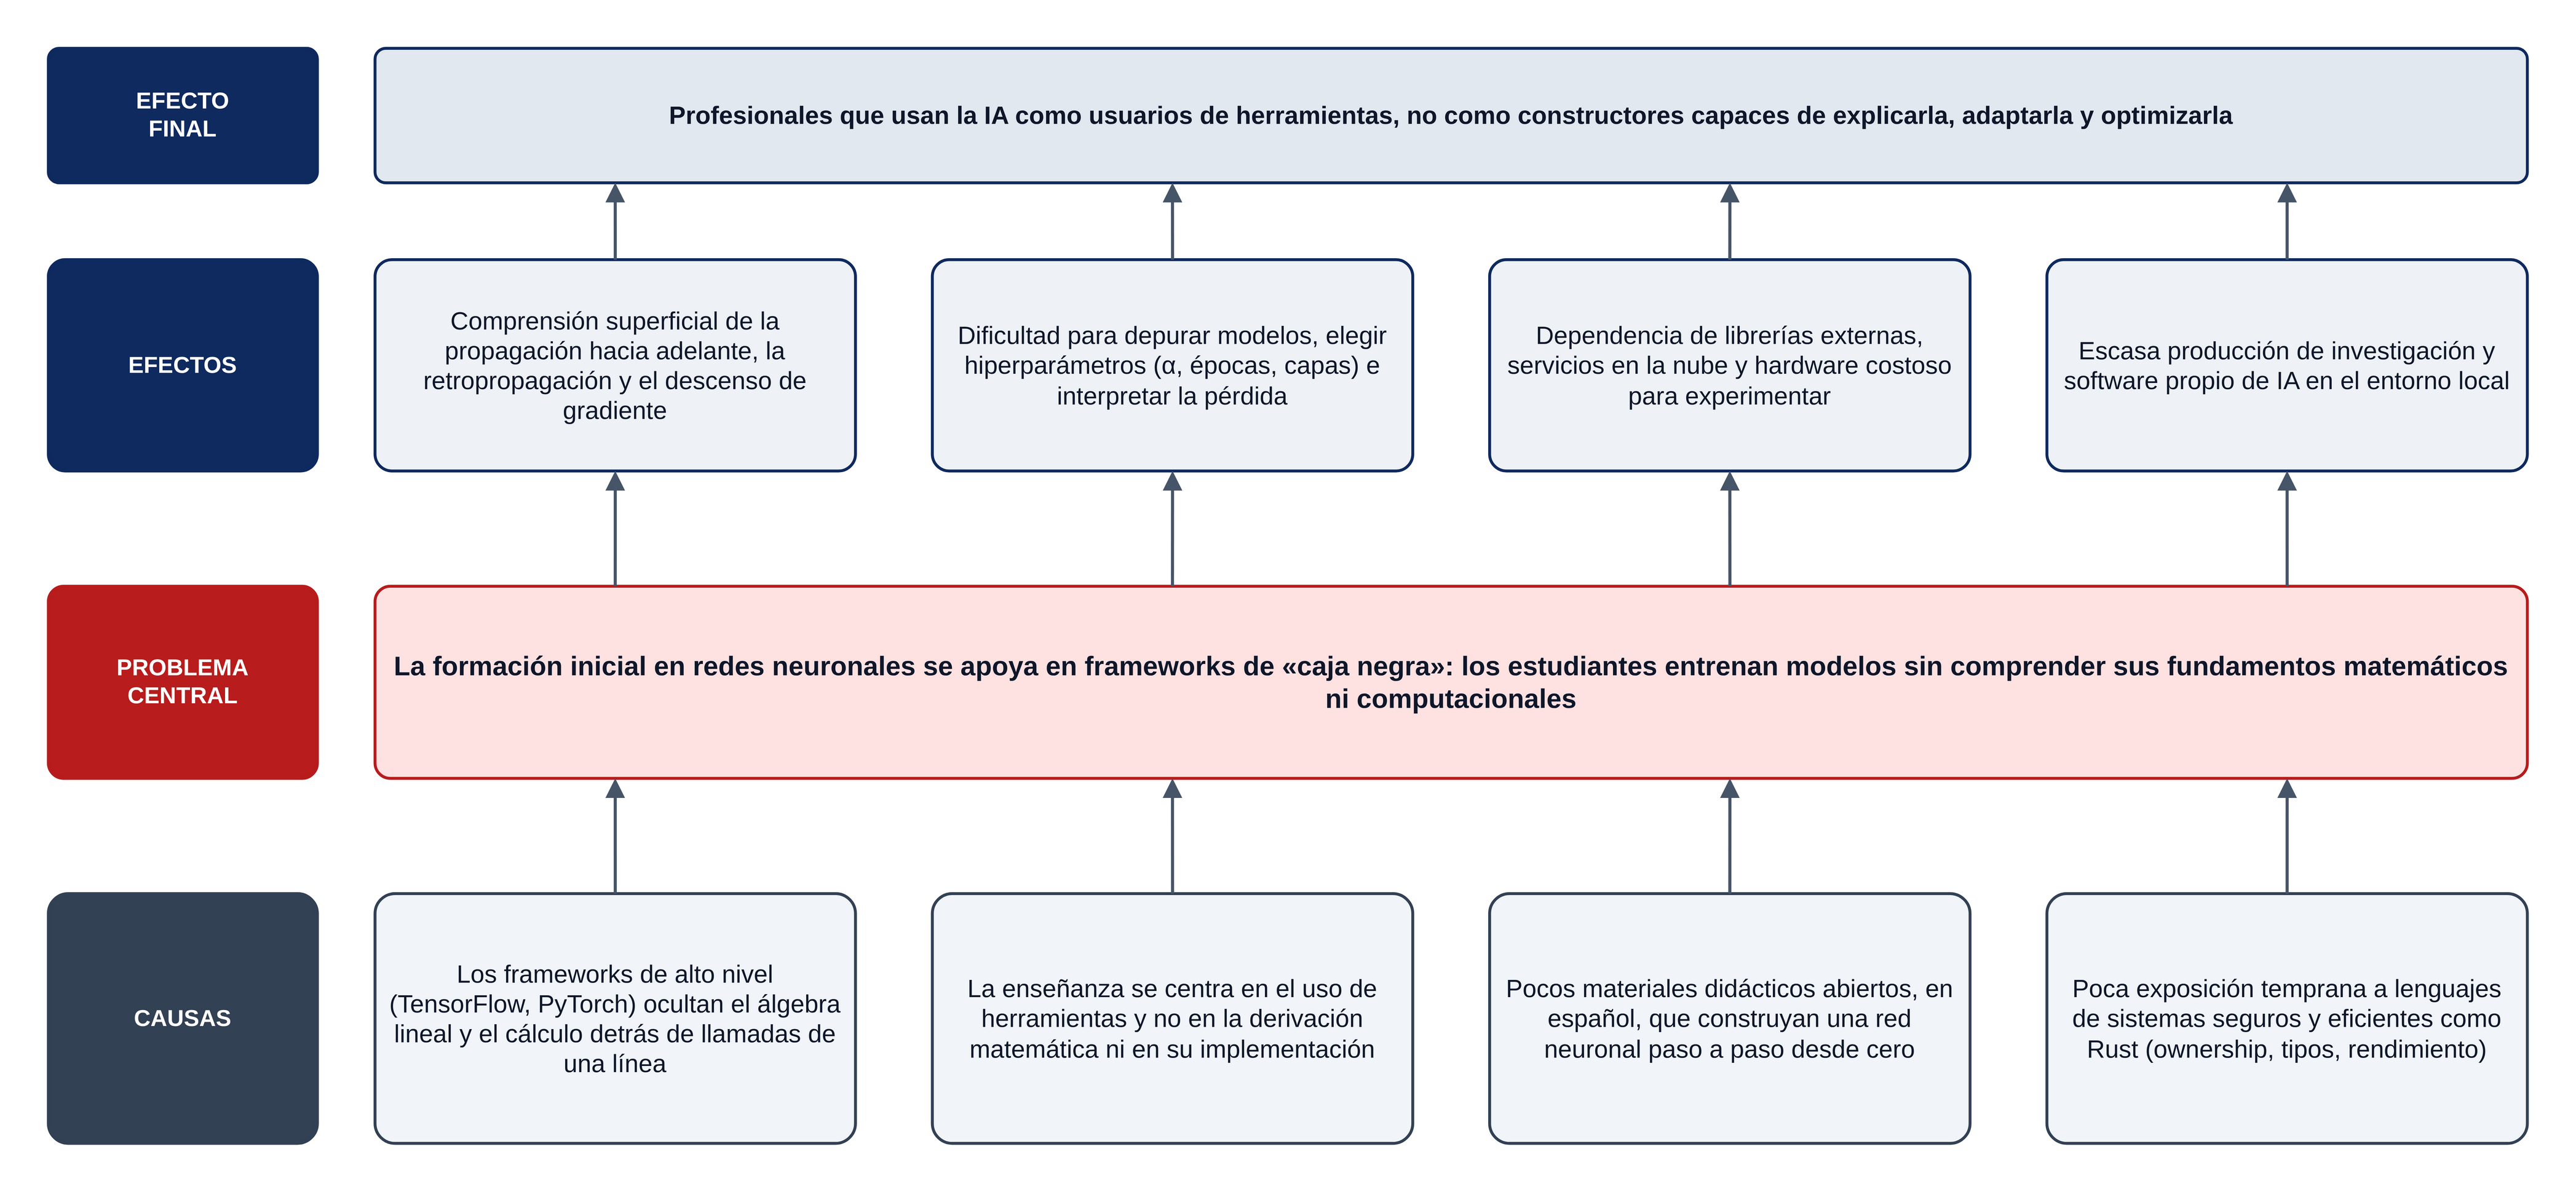
\includegraphics[width=\textwidth,height=0.62\textheight,keepaspectratio]{figuras/diag01_arbol_problemas.png}
\fuente{Las causas se ubican en la parte inferior, el problema central en el centro y los efectos y el efecto final en la parte superior. Diagrama editable: \texttt{diagramas/01\_arbol\_problemas.drawio}.}
\end{figure}

El análisis causal muestra cuatro factores que se refuerzan entre sí. En primer lugar, la enseñanza de la IA se apoya en bibliotecas que encapsulan el álgebra y el cálculo, de modo que el estudiante no necesita ---ni tiene oportunidad de--- implementar una multiplicación matricial o una derivada. En segundo lugar, la matemática de los primeros semestres se presenta de forma desconectada de sus aplicaciones computacionales, por lo que la regla de la cadena o el producto matriz-vector parecen contenidos abstractos sin relación con el software. En tercer lugar, los recursos disponibles suelen exigir equipos con alto poder de cómputo o servicios de pago. En cuarto lugar, las prácticas de programación de los primeros cursos rara vez incorporan pruebas automatizadas y experimentos reproducibles, lo que dificulta distinguir un programa que funciona de uno que parece funcionar. Como efecto, se forman usuarios de herramientas con escasa capacidad para explicar, depurar o adaptar los modelos que utilizan.

\subsection{Pregunta de investigación}
La formulación anterior se concreta en la siguiente pregunta, que guía el diseño de la solución y el análisis de resultados: ¿es posible construir, con fines educativos y sin \emph{frameworks} de aprendizaje automático, una red neuronal artificial en Rust capaz de aprender una relación lineal, clasificar valores booleanos y reconocer patrones visuales simples como las vocales A, E, I, O, U, verificando sus ecuaciones mediante pruebas automatizadas y experimentos reproducibles?

\subsection{Delimitación}
La delimitación establece las fronteras del trabajo para que los resultados se interpreten dentro de su alcance real. En el plano temático, el proyecto aborda redes neuronales densas de propagación hacia adelante (\emph{feedforward}) con funciones de activación Sigmoid, ReLU, lineal y softmax, pérdida de error cuadrático medio y descenso de gradiente. En el plano técnico, la implementación principal es el repositorio oficial del equipo (\url{\Repositorio}), escrito en Rust (edición 2024) sin crates de aprendizaje automático, y se ejecuta en un computador personal convencional. En el plano experimental, se desarrollan tres experimentos de complejidad progresiva ---$y=2x$, clasificación booleana y vocales--- con datos sintéticos definidos en el código fuente, complementados con XOR y vocales con ruido en el motor de validación. Quedan fuera del alcance las redes convolucionales y recurrentes, la aceleración por GPU, el procesamiento de conjuntos de datos masivos y el despliegue en producción.

\section{Justificación}\label{sec:justificacion}
La pertinencia del proyecto se sustenta en cuatro dimensiones complementarias: el valor técnico de la solución, su utilidad académica para la asignatura, su impacto social y educativo, y la viabilidad de su ejecución con los recursos disponibles.

\subsection{Justificación técnica}
Rust ofrece un rendimiento comparable al de C sin recolector de basura y con seguridad de memoria garantizada por el compilador \citep{klabnik2023,jung2018}. Su sistema de tipos y el manejo explícito de errores mediante \texttt{Result} permiten detectar de forma controlada los errores de dimensión que, en otros lenguajes, producirían resultados incorrectos silenciosos o fallos de segmentación. La herramienta \texttt{cargo} integra compilación, pruebas, análisis estático y documentación, lo que facilita una metodología de desarrollo verificable. Prescindir de dependencias externas obliga a implementar cada operación numérica, con la ventaja adicional de que el resultado es un binario pequeño, portable y auditable línea por línea.

\subsection{Justificación académica}
Construir una red neuronal desde cero obliga a traducir cada ecuación matemática en código verificable. Ese ejercicio consolida conocimientos de álgebra lineal (productos matriz-vector, transpuestas, producto de Hadamard), de cálculo diferencial (regla de la cadena y derivadas parciales) y de programación estructurada, y permite comprender por qué funcionan técnicas que en los \emph{frameworks} aparecen como una sola llamada a función \citep{nielsen2015,deisenroth2020}. Para Programación 1, el proyecto ofrece un caso integrador en el que variables, ciclos, funciones, arreglos, estructuras, módulos y pruebas cobran sentido dentro de un sistema completo, como se detalla en el Capítulo~\ref{cap:inf120}.

\subsection{Justificación social y educativa}
El proyecto se publica como código abierto y no requiere hardware especializado, licencias ni conexión permanente a servicios en la nube. Esto lo vuelve accesible para estudiantes de cualquier provincia y lo convierte en un material reutilizable para la enseñanza de la IA en la universidad pública. La prueba de escritorio documentada, las gráficas generadas desde datos reales y la guía de demostración permiten que otros estudiantes reproduzcan los resultados y los utilicen como punto de partida para sus propios proyectos.

\subsection{Viabilidad}
El proyecto es viable porque utiliza exclusivamente herramientas gratuitas (Rust, Cargo, Git, Python con \texttt{matplotlib}, \LaTeX{} y draw.io), se ejecuta en equipos convencionales y se apoya en una bibliografía consolidada. El equipo de cinco integrantes distribuyó el trabajo en fases con entregables verificables, y la validación mediante pruebas automatizadas y experimentos con semilla fija garantiza que cualquier evaluador pueda obtener los mismos resultados \citep{hernandez2018}.

\section{Objetivo general}\label{sec:objgeneral}
El objetivo general orienta la totalidad del proyecto y define el resultado verificable que se espera alcanzar.

\begin{nota}[Objetivo general]
Desarrollar una red neuronal artificial desde cero utilizando el lenguaje Rust, sin \emph{frameworks} de aprendizaje automático ni bibliotecas de álgebra lineal, implementando sus fundamentos matemáticos (álgebra lineal, funciones de activación, función de pérdida, gradientes y descenso de gradiente) y validando su funcionamiento mediante tres experimentos reproducibles y una verificación complementaria con pruebas automatizadas.
\end{nota}

\section{Objetivos específicos}\label{sec:objespecificos}
Los objetivos específicos descomponen el objetivo general en metas concretas y medibles, alineadas con las fases de desarrollo descritas en el Capítulo~\ref{cap:metodologia}. La Tabla~\ref{tab:objetivos} relaciona cada objetivo con su indicador de verificación.

\begin{enumerate}[label=\textbf{OE\arabic*.},leftmargin=3.2em,itemsep=4pt]
\item Implementar estructuras genéricas de vectores y matrices con operaciones de suma, resta, producto punto, multiplicación matricial, producto elemento a elemento, escalamiento y transpuesta, con validación de dimensiones.
\item Implementar las funciones de activación Sigmoid y ReLU, la función softmax, y la función de pérdida de error cuadrático medio (MSE) con su derivada.
\item Construir neuronas, capas densas y una red con propagación hacia adelante, y entrenarlas mediante gradientes y descenso de gradiente; extender la retropropagación a redes con capas ocultas en el motor complementario.
\item Verificar la corrección de las ecuaciones mediante pruebas unitarias, incluida la comparación entre gradientes analíticos y numéricos (\emph{gradient checking}).
\item Ejecutar y analizar tres experimentos progresivos ---regresión $y=2x$, clasificación booleana y reconocimiento de vocales A, E, I, O, U--- y complementarlos con XOR y vocales con ruido, registrando métricas reales en archivos CSV.
\item Medir el rendimiento real (tiempos de ejecución y tamaño del binario) compilado en modo \emph{release}.
\end{enumerate}

\begin{table}[!htbp]
\caption{Matriz de objetivos específicos, indicadores y medios de verificación}\label{tab:objetivos}
\small
\begin{tabularx}{\textwidth}{@{}l >{\raggedright}X >{\raggedright\arraybackslash}X@{}}
\toprule
Objetivo & Indicador verificable & Medio de verificación \\
\midrule
OE1 & Operaciones algebraicas con comprobación de dimensiones & \texttt{src/math/} (oficial) y pruebas de \texttt{math} (complementario) \\
OE2 & Activaciones, softmax y MSE operativas; derivadas verificadas & \texttt{src/neural/}, \texttt{src/learning/} y \emph{gradient checking} \\
OE3 & Neurona, capa y red entrenables; retropropagación multicapa & Experimentos oficiales y motor complementario \\
OE4 & 52 pruebas aprobadas en el motor complementario & Anexo~\ref{anx:tests} \\
OE5 & Métricas reales de los experimentos & \path{resultados/oficial/*.csv}, Capítulo~\ref{cap:implementacion} \\
OE6 & Tiempos de ejecución y tamaño del binario & \path{resultados/oficial/resumen.csv}, \path{benchmarks.csv} \\
\bottomrule
\end{tabularx}
\fuente{Elaboración propia. Los resultados de cada indicador se contrastan en el Capítulo~\ref{cap:conclusiones}.}
\end{table}
